\section{timer.h File Reference}
\label{timer_8h}\index{timer.h@{timer.h}}


This graph shows which files directly or indirectly include this file:\begin{figure}[H]
\begin{center}
\leavevmode
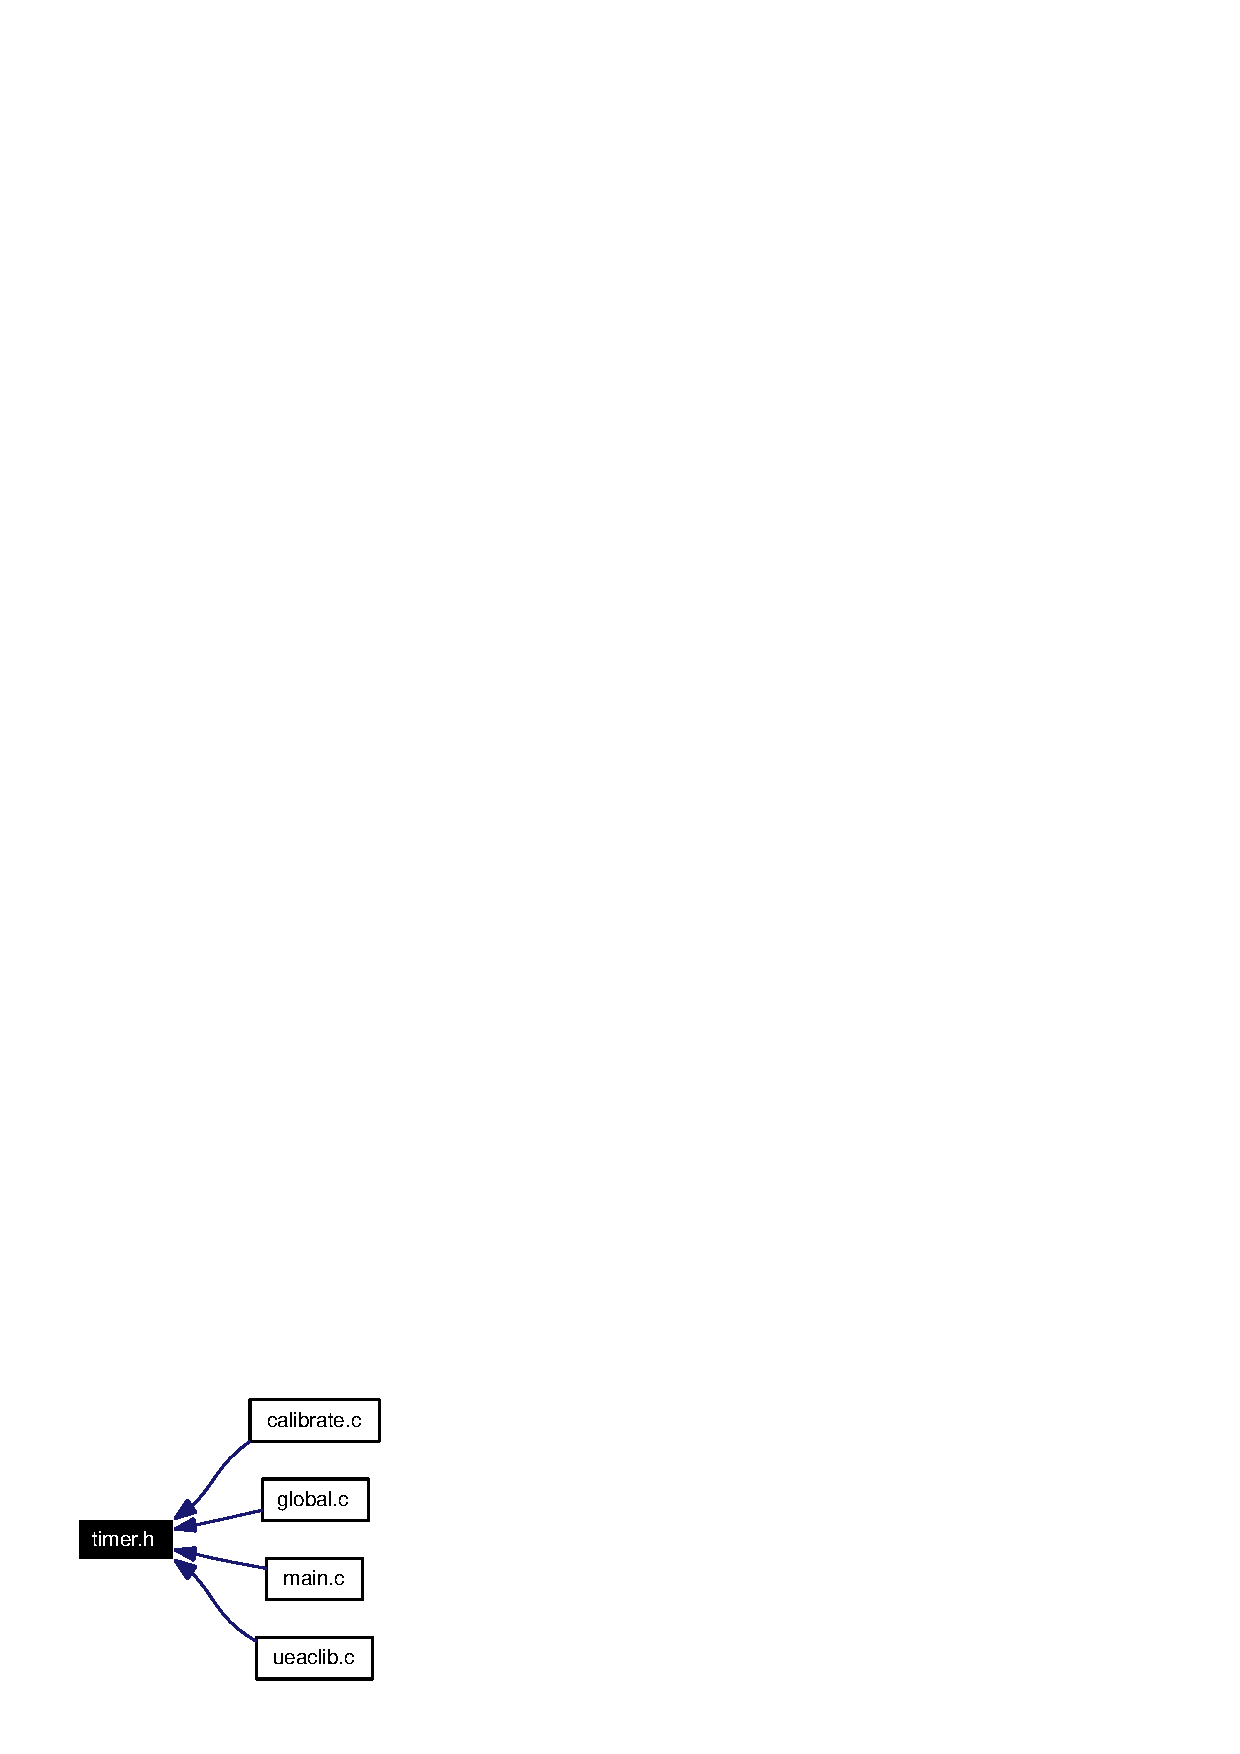
\includegraphics[width=91pt]{timer_8h__dep__incl}
\end{center}
\end{figure}
\subsection*{Functions}
\begin{CompactItemize}
\item 
void {\bf delay\_\-1\_\-25m\-S} (int count)
\end{CompactItemize}


\subsection{Function Documentation}
\index{timer.h@{timer.h}!delay_1_25mS@{delay\_\-1\_\-25mS}}
\index{delay_1_25mS@{delay\_\-1\_\-25mS}!timer.h@{timer.h}}
\subsubsection{\setlength{\rightskip}{0pt plus 5cm}void delay\_\-1\_\-25m\-S (int {\em count})}\label{timer_8h_a0}




Definition at line 116 of file timer.c.

References timer\_\-tick.

Referenced by current\_\-output\_\-calibration(), main(), print\_\-grid\_\-i(), scan\_\-leds(), and scan\_\-probes().

\footnotesize\begin{verbatim}116                              {
117   int tick_counter=0;
118   while (tick_counter<count) {
119     if (timer_tick) {
120       tick_counter++;
121       timer_tick=0;
122     }
123   }
124 }
\end{verbatim}\normalsize 


